

% #######################################################################################################################################
\chapter{Max pooling Implementation}
\label{sec:Appendix-B}
\label{sec:Max pooling}

In \acp{dnn}, there are ``pooling''\cite{stanford_pooling} layers which perform an operation on a region of a feature layer. 
The common pooling operation is max-pooling (see Figure \ref{fig:Baseline DNN showing layer order}) where a group of feature \acp{an} are compared and the \ac{an} with the maximum state value is passed to the next layer.
The feature \acp{an} compared are a 2x2 region as shown in Figure \ref{fig:Pooling 3D layer}.

This work calculates the ``max pooling'' layer by sequencing the \acp{an} calculations such that the pooling \ac{roi} group of features are cascaded.
A maximum comparison operation is performed on the current and previous \ac{an} state and the maximum value retained. After the final comparison, the result is the next layer's \ac{an} state.
This sequencing is shown in Figure \ref{fig:Pooling implementation}.

\begin{figure}[h]
  \centering
  \captionsetup{justification=centering}
  \captionsetup{width=0.9\textwidth}
  \begin{minipage}{1\textwidth}
    \centering
    \centerline{
    \mbox{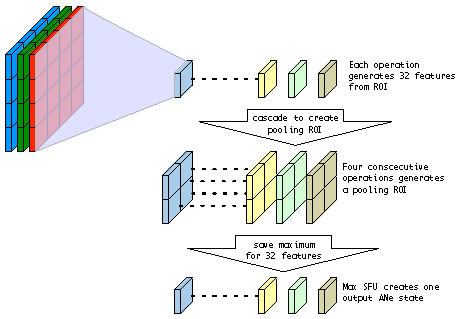
\includegraphics[angle=0, width=.65\textwidth]{pooling3D}}
    }
    \caption{Classifier additional implementation layers}
    \label{fig:Pooling 3D layer}
  \end{minipage}
%\end{figure}

%\begin{figure}[h]
  \bigskip
  \vspace{0.5cm}
  \begin{minipage}{1\textwidth}
    \centering
    \centerline{
    \mbox{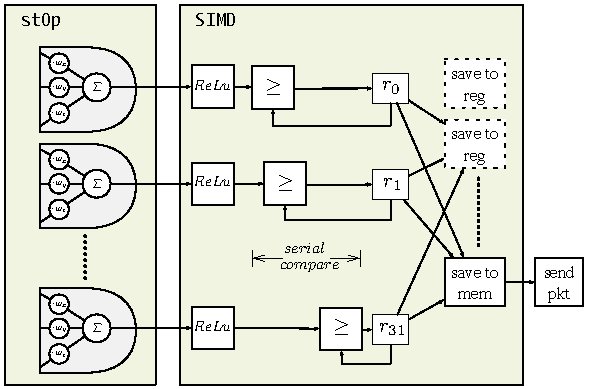
\includegraphics[angle=0, width=.55\textwidth]{poolingImplementation}}
    }
    \caption{Pooling implementation}
    \label{fig:Pooling implementation}
  \end{minipage}
\end{figure}


